\documentclass[12pt]{book}
\usepackage{amsthm}
\usepackage{libertine}
\usepackage{newtxmath}
\usepackage[utf8]{inputenc}
\usepackage[margin=1in]{geometry}
\usepackage{amsmath,amssymb}
\usepackage{multicol}
\usepackage[shortlabels]{enumitem}
\usepackage{siunitx}
\usepackage{cancel}
\usepackage{graphicx}
\usepackage{pgfplots}
\usepackage{listings}
\usepackage{tikz}
\usepackage{tikz-cd}
\usepackage{mathrsfs}
\usepackage{accents}
\usepackage{fancyhdr}

\fancyhf{}
\cfoot{\thepage}
\renewcommand{\headrulewidth}{0pt}
\fancyhead[C]{\rightmark}
\pagestyle{fancy}

\theoremstyle{plain}
\newtheorem{theorem}{Theorem}[section]
\newtheorem{lemma}{Lemma}[section]

\theoremstyle{definition}
\newtheorem{definition}{Definition}[section]
\newtheorem{exercise}{Exercise}[section]
\newtheorem{example}{Example}[section]
\newtheorem*{examples}{Examples}
\newtheorem*{remark}{Remark}
\newtheorem*{remarks}{Remarks}

\newcommand{\dd}[1]{\mathrm{d}#1}
\newcommand{\utilde}[1]{\underaccent{\tilde}{#1}}


\title{
    Linear Systems and Introductory Algebraic Geometry
    
    \begin{Large}
        Interdisciplinary Mathematics -- Volume VIII
    \end{Large}
}
\author{Robert C. Hermann}
\date{1974}

\begin{document}

\maketitle

\section{Preface}

Systems Theory is a good contemporary example of the sort of approach to science that I call Interdisciplinary Mathematics.
It arose in the 1940s and 1950s from work in Electrical and Mechanical Engineering, particularly circuit, communication, and optimal control theory.
It offers a unified mathematical framework to look at (and solve) problems in a wide variety of fields.
Further, this mathematics is not of the traditional sort involved in engineering education but involves virtually every field of modern mathematics.

The attraction for me in this subject is that one sees here an interplay of intuition suggested by interesting applications and the fun force and beauty of modern mathematics, as one used to see in the classical period of mathematical physics.
It would be an interesting historical question to ask why mathematical physics no longer plays a vanguard role.
I suspect it is not intrinsic to the subject (as I tried to show in my earlier books, physics, particularly elementary particle physics, is still extremely rich in generating mathematical ideas and intuition), but is due to certain perverse features of the discipline.
Many leading physicists are smug; a manifestation of this is the poor education of physics students in mathematics, as contrasted say with that of the best engineering students.
Not that physicists don't learn mathematics - my criticism is that they mainly learn outdated or overly `pragmatic' mathematics.
On the other hand, what exists in the way of organized mathematical physics today (typified, say, by the Communications in Mathematical Physics or Journal of Mathematical Physics) carries over the vices of aridity and sterility of contemporary mathematics.
Without sufficiently close contact with the problems arising in mainstream physics, it is often an intellectual stream of physics, made much worse by the rigidity enforced on the scientific world in the last few years by financial troubles.

My interest in Systems Theory is primarily in its mathematical structure, particularly involving algebra and geometry, and in its applications to areas outside of engineering, e.g., in the books by Brockett, Desoer, and Kalman-Arbib-Falb, but done in a way that I believe will be interesting even to experts, since I use Linear Algebra more systematically and efficiently than before. This material would be an excellent topic for a senior or beginning graduate course in mathematics or engineering. I have added expository material on Algebraic Geometry, since, as R. Kalman has emphasized, this area of mathematics is highly relevant to the ultimate development of Systems Theory. Volume IX will develop the ramifications into differential geometry, which is much closer to my own research interest. I will occasionally refer to my other books. ``Volume II'' refers, for example, to the second volume of this interdisciplinary series. The other books are referred to by abbreviations listed in the bibliography. For example, ``LGP'' refers to ``Lie Groups for Physicists.''

Over the years, I have benefited in a general way from conversations on Systems Theory with R. Brockett and R. Kalman, and I would like to thank them. Prof. John Stachel has provided excellent scientific hospitality, inspiration, and working conditions for me as a visitor at the Institute for Relativity Studies of Boston University, and I thank him. Alta Zapf has again typed magnificently.

\chapter{General Ideas of Linear Systems Theory}

\section{Introduction}

The main aim of this volume is the study of the algebraic ideas that enter into the study of linear, time-invariant, finite-dimensional systems.
(Refer to Brockett [1], Desoer [1], Kalman, Arbib and Falb [1], Rosenbrock [1], Zadeh and Desoer [1] for the standard theory.) %TODO: Add reference in the bibliography and don't hard code ref numbers.
In fact, R. Kalman has been the systems theorist who has consistently suggested a program of study of linear systems by means of the tools of algebra, and here I intend to follow his suggestion.

Because it is closest to my own intuition, I shall begin with a differential equation framework for system theory, which of course means that we work over the real or complex numbers as ground field.
However, there are various means of generalization available (e.g. replacing the differential equations by difference equations) that enables one to build systems that work with other fields as scalars.
Additionally, much of automata and coding theory involves similar algebraic ideas, with fields of finite characteristic appearing as the scalar field.

\section{A Definition of a ``System'' in Terms of Differential Equations}

Let $K$ denote the real or complex numbers.
Suppose given three vector spaces (always finite dimensional) over $K$, denoted by
$$U, X \text{ and } Y,$$
with:
\begin{itemize}
    \item $U$ called the \textbf{input space}.
    \item $Y$ called the \textbf{output space}.
    \item $X$ called the \textbf{state space}.
\end{itemize}
Also, let $f, g$ be maps with the following domains and ranges,
\begin{align}
    f: X \times U &\to X \\
    g: X \times U &\to Y.
\end{align}
With this choice of spaces and maps we associate the following system of ordinary differential equations:
\begin{align}
\begin{split} \label{eq:ODESystem1}
    \frac{\dd{x}}{\dd{t}} &= f(x, u) \\
    y(t) &= g(x(t), u(t)).
\end{split}
\end{align}
The ordered 5-tuple
$$\sigma = (U, X, Y, f, g)$$
is said to be a \textbf{system}.

Typical elements of $X, U, Y$ are denoted $x, u, y$. $t$ is a real variable, ranging say over
$$0 \leq t < \infty.$$
A curve
$$t \mapsto (x(t), u(t), y(t)) \in X \times U \times Y$$
is said to be a \textbf{trajectory} of the system if it is a solution of the equations (\ref{eq:ODESystem1}).
The curve $t \mapsto u(t)$ in $U$ is then called the \textbf{input}, the curve $t \mapsto x(t)$ is called the \textbf{state curve}, and the curve $t \mapsto y(t)$ is called the \textbf{output}.

\begin{definition}
    A curve $t \mapsto (u(t), y(t))$ in $U \times Y$ is called an \textbf{input-output pair} if there is a curve $t \mapsto x(t)$ in the state space $X$ such that
    $$t \mapsto (x(t), u(t), y(t))$$
    is a solution of (\ref{eq:ODESystem1}), i.e. is a trajectory of the system.
\end{definition}

One main mathematical goal of systems theory is to study to what extent the set of input-output pairs characterizes the whole system.

\begin{remarks}
\begin{enumerate}
    \item I have chosen this specific mathematical framework for describing what is meant by a "system" so that we can go to work with a minimum of definitions.
    Refer to Kalman, Arbib and Falb [1], Zadeh and Desoer [1], for the full story. % TODO: Move refs to bibliography.
    Of course, one possible generalization is to allow the functions $f( , ), g( , )$ on the right hand side of (\ref{eq:ODESystem1}) to depend on $t$.
    Another generalization would be to allow $X, Y, U$ to be manifolds.
    Such a formulation of systems theory is being developed by Sussman [1]. % TODO: Move refs to bibliography.
    I hope to consider it in another part of this treatise.
    \item It is, of course, useful if the reader is familiar with the areas of application from which this mathematical version of ``systems theory'' arose.
    One such area is electrical circuit theory.
    The book by Anderson and Vongpanitlerd [1] is recommended here. % TODO: Move refs to bibliography.
    There has been widespread discussion in the relevant literature about the possibilities of applying ``systems theoretic'' ideas, of the sort to be described here, to computer science, biology, economics, etc., but I do not know very much about this work, hence will not comment on it.
    Of course, systems theory is very closely related to optimal control theory, and there are many important applications via this connection to economics, mechanical engineering, operations research, etc.
    \item One will find many ways in the engineering literature to describe ``systems'' by means of diagrams.
    Of course, a pictorial representation suggests itself from the ``input'' and ``output'' for the curves $t \mapsto u(t), y(t)$.

    \begin{equation*}
    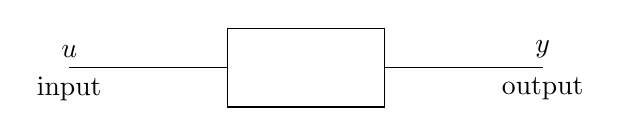
\begin{tikzpicture}
        \node[draw, rectangle, minimum width=2cm, minimum height=1cm] (box) at (0,0) {};
        \draw (box.west) -- ++(-2,0) node[above]{$u$} node[below]{input};
        \draw (box.east) -- ++(2,0) node[above]{$y$} node[below]{output};
    \end{tikzpicture}
    \end{equation*}
    
    In this way of thinking, the ``state'' structure is thought of as a ``black box,'' which is known only via its response to various inputs.
    Here we touch on a very interesting difference in outlook between physics and engineering.
    From the mathematical point of view, much of physics is the study of the pair $(X, \varphi)$ consisting of a ``state space'' $X$, and a one-parameter semi-group of transformations $t \mapsto \varphi(t): X \to X$ acting on $X$.
    If the initial state $x_0 \in X$ is given at $t = 0$, the future
    $$t \mapsto \varphi(t)(x_0)$$
    is known.
    This outlook is clearest, of course, in classical Newtonian mechanics, where $X$ is finite dimensional and $\varphi$ is determined by solving ordinary differential equations, but it carries over also to quantum mechanics, at the expense of making $X$ and $\varphi$ more complicated mathematically.
    This framework suggests the physicist's main job is to ``approximate'' $X$ as best he can, and make predictions to be checked with experiment.
    This implies that there is some physical ``truth'' or ``law'' that the scientist is trying to discover.
\end{enumerate}
\end{remarks}

Let us call the pair $(X, \varphi)$ the \textbf{physicists' dynamical system}.
We can see a difference in outlook between the physicist and engineer by examining the difference between $(X, \varphi)$, and a ``system''
$$(X, Y, U, f, g).$$
Mathematically, we compare
\begin{align} \label{eq:PhysDynSys1}
    \frac{\dd{x}}{\dd{t}} &= \varphi(x(t))
\end{align}
and
\begin{align}
\begin{split} \label{eq:ODESystem2}
    \frac{\dd{x}}{\dd{t}} &= f(x(t), u(t)) \\
    y(t) &= g(x(t), u(t)).
\end{split}
\end{align}
Of course, (\ref{eq:ODESystem2}) can be constructed to reduce to (\ref{eq:PhysDynSys1}) as a special case.
However, what is basically different is the outlook -- the input curve $t \mapsto u(t)$ is to be chosen so as to achieve \textbf{some desired properties of the output curve} $t \mapsto y(t)$.
Discovering the precise ``nature'' of the state-mechanism, i.e., the functions $f$ and $g$, is not so important as in physics.
One then gives up the deeply satisfying feeling one gets from studying physics that one is trying to discover deep ``truths,'' and instead puts the emphasis on desired ends.
One might say then that ``systems theory'' is the right mathematics for technology and social phenomena.
I am not sufficiently learned in the philosophy of science to go into these distinctions in any greater depth or detail, but it is clear in my mind that it would be worthwhile to do so -- in fact, it might even give us vastly expanded insights into the times we live in.

Returning to the mathematics of systems theory, we shall, for the rest of the chapter at least, deal with the only sort that is completely mathematically tractable at the moment, the linear, time-invariant ones.
This means that $f, g$, considered as maps
\begin{align*}
\begin{split}
    f: X \times U &\to X \\
    g: X \times U &\to Y
\end{split}
\end{align*}
between vector spaces, are \textbf{linear} maps.
($X \times U$ is considered to be the direct sum of the vector spaces $X$ and $U$). Thus, $f$ and $g$ are of the following form:
\begin{align}
\begin{split}
    f(x, u) &= Ax + Bu \\
    g(x, u) &= Cx + Du,
\end{split}
\end{align}
where $A: X \to X, B: U \to X, C: X \to Y, D: U \to Y$ are linear maps.
Such a system can then be characterized by
$$(X, U, Y, A, B, C, D).$$
We shall develop the algebraic tools needed to understand the ``structure'' of these linear systems.
They mainly involve linear algebra of a more-or-less standard sort, but -- as R. Kalman emphasizes -- lead one also into problems which are closely related to current pure mathematics research in algebraic geometry and algebraic group theory.

\section{Equivalent and Linearly Equivalent Linear, Time-Invariant Systems}

Let us recapitulate the notation.
$K$ is the field of either the real or complex numbers.
(I shall sketch in a moment how replacing ``differential'' by ``difference'' equations enables one to replace $K$ by more general scalar fields.)
$X, U, Y$ are vector spaces,
\begin{align*}
\begin{split}
    A: X &\to X \\
    B: U &\to X \\
    C: X &\to Y \\
    D: U &\to Y
\end{split}
\end{align*}
are linear maps.
Denote the whole collection by:
\begin{align} \label{eq:sigma1}
    \sigma &= (U, X, Y, A, B, C, D).
\end{align}
We shall call such a $\sigma$ a \textbf{linear system}. The set of all such $\sigma$, with given $U, X, Y$, is denoted by
$$\Sigma.$$
All the data necessary to define a linear system may be summarized in the following diagram of vector spaces and linear maps.
(Note that it is not a ``commutative'' diagram.)

\begin{equation*}
\begin{tikzcd}
    U \ar[r,"D"] \ar[d,"B"'] & Y \\
    X \ar[r,"A"'] & X \ar[u,"C"']
\end{tikzcd}
\end{equation*}

With $\sigma$ given by (\ref{eq:sigma1}), we can consider the following system of linear constant-coefficient equations:
\begin{align}
\begin{split} \label{eq:LinearODESystem1}
    \frac{\dd{x}}{\dd{t}}(t) &= Ax(t) + Bu(t) \\
    y(t) &= Cx(t) + Du(t).
\end{split}
\end{align}

Here is the terminology that goes along with these equations.
$X$ is called the \textbf{state space}.
A typical element is denoted by $x$.

$U$ is called the \textbf{input space}.
A typical element of $U$ is denoted by $u$.
A curve $\utilde{u}: t \mapsto u(t), -\infty < t < \infty,$ in $U$ is called an \textbf{input curve}.

$Y$ is called the \textbf{output space}.
A typical element is denoted by $y$.
A curve $\utilde{y}: t \mapsto y(t)$ is called an \textbf{output curve}.

$\utilde{U}$ and $\utilde{Y}$ denote the space of input and output curves.

\begin{definition}
    An element $(\utilde{u}, \utilde{y}) \in \utilde{U} \times \utilde{Y}$ is called an \textbf{input-output pair} if there is a curve $t \mapsto x(t)$ in the state space $X$, such that the curves $t \mapsto (x(t), u(t), y(t))$ satisfy equation (\ref{eq:LinearODESystem1}).
\end{definition}

Two linear systems $\sigma, \sigma'$ are said to be \textbf{equivalent} if they have the same set of input-output pairs.

\begin{remark}
    To replace (\ref{eq:LinearODESystem1}) by difference equations, let $t$ denote an element of the additive semigroup $\mathbb{Z}_+$, the non-negative integers.
    An input or output curve is now a map
    \begin{align*}
    \begin{split}
        t \mapsto u(t) &\text{ of } \mathbb{Z}_+ \to U \\
        t \mapsto y(t) &\text{ of } \mathbb{Z}_+ \to U.
    \end{split}
    \end{align*}
    Replace $\frac{\dd{u}}{\dd{t}}$ by
    $$\Delta u(t) = u(t + 1) - u(t).$$
    Thus, (\ref{eq:LinearODESystem1}) may be interpreted as a set of difference equations:
    \begin{align*}
    \begin{split}
        \Delta u(t) &= Ax(t) + Bu(t) \\
        y(t) &= Cx(t) + Du(t).
    \end{split}
    \end{align*}
    A further generalization might involve putting a ``delay'' in the differential or difference equations.
    However, we shall work with the differential equation set-up, as the most familiar (at least to me).
\end{remark}

We shall now discuss one concrete way of realizing equivalence of two linear systems with the same $X, U, Y$.
Let $\mathrm{GL}(X)$ denote the space of invertible linear maps
$$g: X \to X.$$
Given $t \mapsto (x(t), u(t), y(t))$ which is a solution of (\ref{eq:LinearODESystem1}), set:
$$x_1(t) = gx(t).$$
Then,
\begin{align}
\begin{split} \label{eq:DifferenceEquationSystem1dx/dt}
    \frac{\dd{x_1}}{\dd{t}} = g\frac{\dd{x}}{\dd{t}} &= g(Ax + Bu) \\
    &= A_1x_1 + B_1u,
\end{split}
\end{align}
with:
\begin{align}
    A_1 &= gAg^{-1} \\
    B_1 &= gB.
\end{align}
Also,
\begin{align}
\begin{split} \label{eq:DifferenceEquationSystem1y}
    y(t) &= Cg^{-1}x_1 + Du \\
    &= C_1x_1 + D_1u
\end{split}
\end{align}
with:
\begin{align}
    C_1 &= Cg^{-1}, \label{eq:C1,1} \\
    D_1 &= D.
\end{align}

We see that equations (\ref{eq:DifferenceEquationSystem1dx/dt}) and (\ref{eq:DifferenceEquationSystem1y}) define a new linear time invariant system
$$\sigma_1 = (U, X, Y, A_1, B_1, C_1, D_1).$$
We see that $\sigma$ and $\sigma_1$ automatically have the same set of input-output pairs, i.e. define equivalent systems.

Let us formalize this construction.

\begin{definition}
    Let $\sigma = (A, B, C, D)$ and $\sigma_1 = (A_1, B_1, C_1, D_1)$ be two linear systems with the same state, input, and output space.
    They are said to be \textbf{algebraically equivalent} if and only if there is a
    $$g \in \textrm{GL}(V)$$
    such that:
    \begin{align}
    \begin{split}
        A_1 &= gAg^{-1} \\
        B_1 &= gB \\
        C_1 &= Cg^{-1} \\
        D_1 &= D.
    \end{split}
    \end{align}
\end{definition}

Our discussion above proves the following (trivial) result:
\begin{theorem}
    If $\sigma = (A, B, C, D)$ and $\sigma_1 = (A_1, B_1, C_1, D_1)$ are algebraically equivalent, then they are equivalent.
\end{theorem}

\begin{remark}
    Sufficient conditions that ``equivalence'' implies ``algebraic equivalence'' are discussed by Brockett [1] and Desoer [1]. % TODO: Add actual citations to bibliography.
    Roughly if the systems are ``minimal'' (in the sense of having a minimal dimensional state space) then the two notions coincide.
    We shall deal with this later.
\end{remark}

We can now reformulate ``algebraic equivalence'' in a more standard group-theoretic way.
Let $\Sigma = \{\sigma\}$ denote the collection of linear systems
$$\sigma = (A, B, C, D).$$
In other work, % TODO: Is this a typo?
\begin{align} \label{eq:Sigma1}
    \Sigma &= L(X, X) \times L(U, X) \times L(X, Y) \times L(U, Y).
\end{align}

\begin{remark}
    In (\ref{eq:Sigma1}), I use the notation from linear algebra, e.g. from volume II. If $V, W$ are vector spaces,
    $$L(V, W)$$
    denotes the vector space of linear maps $V \to W$.
\end{remark}

Let $\mathrm{GL}(X)$ be the group of invertible linear maps $X \to X$.
Let $\mathrm{GL}(X)$ act on $\Sigma$ as follows:

If $g \in \mathrm{GL}(X)$, and
$$\sigma = (A, B, C, D) \in \Sigma,$$
then
\begin{align} \label{eq:gsigma1}
    g\sigma &= (gAg^{-1}, gB, Cg, D).
\end{align}

\begin{exercise}
    Show that (\ref{eq:gsigma1}) defines an action of $\mathrm{GL}(X)$ on $\Sigma$ as a transformation group.
\end{exercise}

Let us restate things in the following way.

\begin{theorem}
    Two linear systems $\sigma, \sigma' \in \Sigma$ are algebraically equivalent if and only if they are on the same orbit of $\mathrm{GL}(X)$ acting on $\Sigma$ via the transformation group action (\ref{eq:gsigma1}).
    Hence, the equivalence classes of linear systems under the equivalence relation defined by ``algebraic equivalence'' are in one-one correspondence with the orbit space
    \begin{align} \label{eq:OrbitSpace1}
        \mathrm{GL}(X)\backslash\Sigma \equiv \{\mathrm{GL}(X)\sigma : \sigma \in \Sigma\}.
    \end{align}
\end{theorem}

We conclude from these remarks that the study of the geometric and algebraic properties of the orbit space (\ref{eq:OrbitSpace1}) might be in close rapport with the properties of elements of $\Sigma$ that are interesting from an engineering point of view.
In this chapter we shall pursue these interconnections.

\begin{remark}
    Notice that the $D$ component of the system $\sigma = (A, B, C, D)$ plays no role in algebraic equivalence, hence it can usually be left out, i.e. be set equal to zero.
\end{remark}

\section{Impulse Response and Transfer Functions; Observability and Controllability}

The differential equations governing linear, time-invariant, ``lumped parameter'' systems, i.e. those of form (\ref{eq:LinearODESystem1}), are relatively easy to handle.
In fact, an explicit solution can be written down for them.
These explicit solutions involve what are called ``impulse responses'' and ``transfer functions'' in the engineering literature.
(Brockett [1] follows terminology introduced by Kalman and gives the name ``weighting pattern'' to what we call ``impulse response.'') % TODO: Add ref to bibliography.

Suppose $\sigma = (A, B, C, D)$ is a system, whose input-output response is governed by the equations (\ref{eq:LinearODESystem1}).
We can, of course solve equations (\ref{eq:C1,1}) explicitly by means of the variation-of-parameter technique and the operator exponential
\begin{align}
    e^{tA} &= 1 + tA + \frac{t^2A}{2} + \dots
\end{align}
(see Vol. III).

Here are the equations:
\begin{align}
    \frac{\dd{x}}{\dd{t}} &= Ax + Bu \label{eq:LinearODESystemdxdt1} \\
    y &= Cx + Du. \label{eq:LinearODESystemy1}
\end{align}
The solution to (\ref{eq:LinearODESystemdxdt1}) is:
\begin{align}
    x(t) &= \int_0^t e^{A(t-s)}Bu(s)\ \dd{s} + e^{At}x(0).
\end{align}
Hence, the complete solution to the system (\ref{eq:LinearODESystemy1}) is:
\begin{align} \label{eq:LinearODESystemy1Solution1}
    y &= \int_0^t Ce^{A(t-s)}Bu(s)\ \dd{s} + Ce^{At}x(0) + Du.
\end{align}

\begin{definition}
    The function
    \begin{align} \label{eq:ImpulseResponse1}
        t &\mapsto Ce^{At}B: R \to L(U, Y)
    \end{align}
    is called the \textbf{impulse response} for the system $\sigma = (A, B, C, D)$.
    Its Laplace transform
    \begin{align} \label{eq:FreqResponse1}
        s &\mapsto C(a-s)^{-1}B
    \end{align}
    is called the \textbf{frequency response} of the system.
\end{definition}

\begin{remarks}
\begin{enumerate}
    \item \textbf{Resolvents}.
    In functional analysis, the operator-valued function
    $$s \mapsto (A-s)^{-1}$$
    is called the \textbf{resolvent} of the operator $A$.
    See Dunford and Schwartz [1], Kato [1], Yosida [1], Reed and Simon [1]. % TODO: Add refs to bibliography.
    Its theory, for operators in infinite dimensional space, plays a big role in mathematical physics and Lie group harmonic analysis.
    See LMP, vol. II, and PALG.
    Of course, the traditional problems of control theory involve a finite dimensional state space $X$ (or at least this is the only situation for which a complete theory exists), but presumably a pursuit of the ultimate ramification and application of systems theory will eventually involve infinite dimensional situations in a critical way.
    \item \textbf{Rational mappings}.
    Since one of our aims is to develop the algebro-geometric foundations of systems theory, it is interesting to ask what kind of an abstract ``object'' the transfer function, given by (\ref{eq:FreqResponse1}), actually is.
    Of course, we can regard it as a mapping in the ordinary sense, by deleting from our ground field, (in this case, the complex numbers $\mathbb{C}$) the eigenvalues of $A$, and regarding (\ref{eq:FreqResponse1}) as a mapping:
    $$C - (\text{eigenvalues of } A) \to L(U, Y).$$
    I do not regard this as a completely satisfactory answer, since it says nothing very precise about what happens at the singular points of the mapping, i.e. the eigenvalues of $A$.
    Algebraic geometry provides us with a ``language'' to discuss (\ref{eq:FreqResponse1}), as a ``rational'' mapping
    $$C \to L(U, Y).$$
    Indeed, this may be the chief reason for introducing algebra-geometric ideas into systems theory.
    \item \textbf{Generalizations to other scalar fields}.
    As (\ref{eq:ImpulseResponse1}) shows, the impulse response does not involve ``algebraic'' functions, while the transfer function does.
    Thus, discussing algebraic objects like the transfer function over other scalar fields than the complex numbers might be a useful generalization.
    For example, it might be relevant to situations where the differential equations were replaced by difference equations.
\end{enumerate}
\end{remarks}

Here is a main result.

\begin{theorem} \label{thm:Equivalence1}
    Let $\sigma = (U, X, Y, A, B, C, D), \sigma_1 = (U, X_1, Y, A_1, B_1, C_1, D_1)$ be two linear systems which have the same input and output vector space, $U$ and $Y$, but possibly different state spaces $X$ and $X_1$.
    Suppose that they are equivalent, in the sense of having the same input and output pairs.
    Then,
    \begin{align}
        C(A-s)^{-1}B &= C_1(A_1-s)^{-1}B_1, \forall s \in \mathbb{C},
    \end{align}
    i.e. they have the same frequency responses.
    Also,
    \begin{align}
        D &= D_1.
    \end{align}
\end{theorem}

\begin{proof}
    Let $t \mapsto u(t)$ be an input curve, and let $x(0)$ be an initial state vector. Let $t \mapsto y(t)$ be the output curve determined by $\{t \mapsto u(t), x(0)\}$ in system $\sigma$. Using (\ref{eq:LinearODESystemy1Solution1}), $y(t)$ is determined by the following formula:
    \begin{align} \label{eq:LinearODESystemy1Solution2}
        y(t) &= \int_0^t Ce^{A(t-s)}Bu(s)\ \dd{s} + Ce^{At}x(0) + Du(t).
    \end{align}
    
    By hypothesis, $\sigma$ and $\sigma_1$ are equivalent.
    This means that there must be a state vector $x_1(0) \in X_1$, such that $\{t \mapsto u(t), x_1(0)\}$ determines the output $t \mapsto y(t)$ in the $c_1$ system, i.e. that:
    \begin{align} \label{eq:LinearODESystemy1Solution3}
        y(t) &= \int_0^t C_1e^{A_1(t-s)}B_1u(s)\ \dd{s} + C_1e^{A_1t}x_1(0) + D_1u(t).
    \end{align}
    Equating (\ref{eq:LinearODESystemy1Solution2}) and (\ref{eq:LinearODESystemy1Solution3}), we have:
    \begin{align} \label{eq:LinearODESystemy1Solution4}
        0 &= \int_0^t \left[Ce^{A(t-s)}B-C_1e^{A_1(t-s)}B_1\right]u(s)\ \dd{s} + Ce^{A_0t}x(0) - C_1e^{A_1t}x_1(0) + (D-D_1)u(t).
    \end{align}
    
    Let us recapitulate the logic which led to equation (\ref{eq:LinearODESystemy1Solution4}).
    The input curve $t \mapsto u(t)$, in $U$ and the state vector $x(0) \in X$ is given.
    $x_1(0)$ is a vector in $X_1$ such that (\ref{eq:LinearODESystemy1Solution4}) holds for all $t$.
    Let us now put in special inputs and states.
    For example:
    \begin{align}
    \begin{split} \label{eq:SpecialInputsStates1}
        u(t) &= e^{-\lambda t}u(0) \\
        x(0) &= 0,
    \end{split}
    \end{align}
    where $\lambda$ is a complex number, $u(0)$ an arbitrary element of $U$.
    Now,
    \begin{align}
    \begin{split} \label{eq:Integral1}
        \int_0^t e^{A(t-s)}e^{-s}\ \dd{s} &= e^{At}\int_0^t e^{-s(A+\lambda)}\ \dd{s} \\
        &= \left.e^{At}(-1)(A+\lambda)^{-1}e^{-s(A+\lambda)}\right|_{s=0}^t \\
        &= -e^{At}(A+\lambda)^{-1}(e^{-t(A+\lambda)} - 1) \\
        &= e^{At}(A+\lambda)^{-1}(e^{At}-e^{-\lambda t}).
    \end{split}
    \end{align}
    Substituting (\ref{eq:LinearODESystemy1Solution4}) into (\ref{eq:SpecialInputsStates1}), and using (\ref{eq:Integral1}) we have:
    \begin{align}
    \begin{split}
        0 &= C(A+\lambda)^{-1}(e^{At}-e^{-\lambda t})Bu(0) - C_1(A_1+\lambda)^{-1}(e^{A_1t}-e^{-\lambda t})B_1u(0) \\
        &+ C_1e^{A_1t}x_1(0) + (D-D_1)u(0).
    \end{split}
    \end{align}
    We see that the coefficients of $e^{-\lambda t}$ in relation (\ref{eq:SpecialInputsStates1}) must vanish, hence:
    \begin{align}
        C(A+\lambda)^{-1}B &= C_1(A_1+\lambda)^{-1}B_1.
    \end{align}
    This says that the frequency response functions are equal, hence proves Theorem \ref{thm:Equivalence1}.
\end{proof}

\begin{remark}
    We can interpret this result in the following way.
    Let $\Sigma$ be the space of linear systems with given input and output spaces $U, Y$.
    Let $E$ be the equivalence relation on $\Sigma$ defined by saying that two systems are the same if they have the same set of input-output pairs.
    Let
    $$\textrm{RM}(C, L(U, Y))$$
    be the space of rational maps: $C \to L(U, Y)$.
    (Later on, after presenting the relevant ideas from algebraic geometry, we shall define $\textrm{RM}$ precisely.)
    Thus, the ``frequency response'' construction defines a map
    \begin{align} \label{def:FrequencyResponseMap1}
        \textrm{FR}: \Sigma &\to \textrm{RM}(C, L(U, Y)).
    \end{align}
    Theorem \ref{thm:Equivalence1} says that this map is constant on the equivalence classes of $E$, hence the map (\ref{def:FrequencyResponseMap1}) passes to the quotient to define a map
    \begin{align}
        \textrm{FR}: E\backslash\Sigma \to \textrm{RM}(C, L(U, Y)).
    \end{align}
    The properties of this map will be one of our main concerns.
\end{remark}

Now we turn to the discussion of the type of system -- the ``completely controllable and observable'' ones -- for which equivalence implies algebraic equivalence.

\section{Completely Controllable and Observable Systems}
Let $\sigma$ be a linear system, described by the following diagram of spaces and mappings

\begin{equation}
\begin{tikzcd} \label{diag:LinearSystem1}
    U \ar[r,"D"] \ar[d,"B"'] & Y \\
    X \ar[r,"A"'] & X \ar[u,"C"']
\end{tikzcd}
\end{equation}

\begin{definition}
    $\sigma$ is said to be \textbf{completely controllable} if the following condition is satisfied:
    \begin{align}
        X &= B(U) + AB(U) + A^B(u) + \dots
    \end{align}
    $\sigma$ is said to be \textbf{completely observable} if the following condition is satisfied.
    \begin{align} \label{eq:CompletelyObservableCondition1}
        \text{Given non-zero } x \in X, \text{ there is an integer } n \text{ such that } \textrm{CA}^n(x) &\neq 0.
    \end{align}
    Alternatively, one may say that:
    \begin{align} \label{eq:CompletelyObservableCondition2}
        \ker(C) \cap \ker(CA) \cap \dots \cap  \ker(CA^n) \cap \dots &= 0.
    \end{align}
\end{definition}

\begin{remark}
    The practical and theoretical meaning of conditions () and () is extensively discussed in the treatises, e.g. Brockett [1], Desoer [1] and Kalman, Arbib, and Falb [1]. % TODO: Add refs in bibliography
    Recall that (\ref{diag:LinearSystem1}) means that, given $x_0, x_1 \in X$, an input curve $t \mapsto u(t), a \leq t \leq b$ can be chosen so that the solution of the equation:
    $$\frac{\dd{x}}{\dd{t}} = Ax + Bu(t)$$
    goes from $x_0$ to $x_1$ as $t$ varies from $a$ to $b$.
    In volume III I have given a brief ``functional analysis'' proof of this fact.
    A differential geometric proof (which I regard as more profound because it extends to non-linear systems) is presented in DGCV.
    As we shall see later on, ``complete observability'' is ``dual'' to controllability.
\end{remark}

Here is a main result.

\begin{theorem} \label{thm:Equivalence2}
    Let $\sigma = (A, B, C, D), \sigma_1 = (A_1, B_1, C_1, D_1)$ be completely observable linear systems, with the same input, output and state spaces.
    Suppose $\sigma$ and $\sigma_1$ are equivalent. Then, $\sigma$ and $\sigma_1$ are algebraically equivalent.
\end{theorem}

\begin{proof}
    Let $t \mapsto u(t), y(t)$ be an input-output curve for the system $\sigma$.
    By (\ref{eq:LinearODESystemy1Solution2}), this means that there is an $x_0 \in X$ such that
    \begin{align} \label{eq:CompletelyObservableLinearODESystemy1}
        y(t) &= \int_0^t Ce^{A(t-s)}Bu(s)\ \dd{s} + Ce^{At}x_0 + Du(t).
    \end{align}
    To say that $\sigma$ is equivalent to $\sigma_1$ is to say that $t \mapsto (u(t), y(t))$ is also an input-output curve for the system $\sigma_1$, i.e. that there is an $x_1 \in X$ such that:
    \begin{align} \label{eq:CompletelyObservableLinearODESystemy2}
        y(t) &= \int_0^t C_1e^{A_1(t-s)}Bu(s)\ \dd{s} + C_1e^{A_1t}x_1 + D_1u(t).
    \end{align}
    Now, by Theorem \ref{thm:Equivalence1}, $\sigma$ and $\sigma_1$ have the same frequency response function.
    Hence, they have the same impulse response function (since ``frequency response'' is the Laplace transform of ``impulse response'', and the Laplace transform is a one-one map), i.e. the first terms on the right hand sides of (\ref{eq:CompletelyObservableLinearODESystemy1}) and (\ref{eq:CompletelyObservableLinearODESystemy2}) are equal.
    Hence, we have:
    \begin{align}
        Ce^{At}x_0 + Du(t) &= C_1e^{A_1t}x_1 + D_1u(t).
    \end{align}
    Now, $t \mapsto u(t)$ may be an \emph{arbitrary} curve in the input space $U$. $(D-D_1)$ is a linear map
    $$U \to Y.$$
    It should be intuitively clear that the image of an arbitrary curve in $U$ under the linear map $D-D_1$ is the sum of exponentials if and only if $D-D_1=0$, i.e.
    \begin{align} \label{eq:D=D_1}
        D &= D_1.
    \end{align}
\end{proof}

\begin{exercise}
    Give the details of the proof of (\ref{eq:D=D_1}).
\end{exercise}

With (\ref{eq:D=D_1}) satisfied, everything reduces to the following identity:
\begin{align} \label{eq:Ce^(At)x_0=C_1e^(A_1t)x_1}
    Ce^{At}x_0 &= C_1e^{A_1t}x_1.
\end{align}
Using the power-series expansion of $e^{At}$, (\ref{eq:Ce^(At)x_0=C_1e^(A_1t)x_1}) implies the following series of algebraic identities:
\begin{align} \label{eq:AlgebraicIdentities1}
    CA^n(x_0) &= C_1A_1^n(x_1) \text{ for } n = 0, 1, \dots
\end{align}
Now, change the logic somewhat, and suppose the input curve $t \mapsto u(t)$ and the state vector $x_0 \in X$ are given.
Define the output $t \mapsto y(t)$ of $\sigma$ by formula (\ref{eq:CompletelyObservableLinearODESystemy1}).
Here is the diagram for this:

\begin{equation}
\begin{tikzpicture} \label{diag:x_0}
    \node[draw, rectangle, minimum width=1cm, minimum height=1cm] (box) at (0,0) {};
    \node[above] (x0) at (box.north) {$x_0$};
    \node[above] at (x0.north) {state};
    \draw (box.west) -- ++(-2,0) node[above]{$u$};
    \draw (box.east) -- ++(2,0) node[above]{$y$};
\end{tikzpicture}
\end{equation}

In words, we set the ``dial'' in the ``black-box'' represented by $\square$ so that it is in state $x_0$, and read the output curve $t \mapsto y(t)$.

Now, note that ``complete observability'' of $\sigma_1$ implies that $x_1$ is completely determined by $x_0$ and condition (\ref{eq:AlgebraicIdentities1}).
For, if $x_1^1$ were another element of $X$ such that
$$CA^n(x_0) = C_1A_1^n(x_1^1) \text{ for all } n,$$
then
$$C_1A_1^n(x_1^1-x_1) = 0 \text{ for all } n,$$
which, by (\ref{eq:CompletelyObservableCondition1}), implies
$$x_1^1 = x_1.$$

Let us now run the ``machine'' represented by (\ref{diag:x_0}) with zero input, and given initial state $x_0$.
There is then an $x_1$ such that (\ref{eq:AlgebraicIdentities1}) is satisfied, which is uniquely determined by $x_0$. We can then define a map
$$g: X \to X$$
so that:
\begin{align} \label{eq:g(x_0)=x_1}
    g(x_0) &= x_1.
\end{align}
Since $x_1$ is uniquely determined by $x_0$, and the conditions (\ref{diag:x_0}) (regarded as an equation for $x_1$) are linear, the map $g$ is linear. % TODO: Is this reference a typo?
Thus, $g$ satisfies the following conditions:
\begin{align} \label{eq:CA^n=C_1A_1^ng}
    CA^n &= C_1A_1^ng \text{ for all } n.
\end{align}
In particular,
\begin{align} \label{eq:C=C_1g}
    C &= C_1g.
\end{align}
Complete observability of $\sigma$ implies $g$ is one-one.
For, if
$$gx = 0,$$
(\ref{eq:CA^n=C_1A_1^ng}) is used to imply
$$CA^nx = 0 \text{ for all } n,$$
and (\ref{eq:CompletelyObservableCondition1}) implies $x = 0$.
Finite dimensionality of $X$ and linearity of $g$ now implies that $g^{-1}$ exists.
To prove:
\begin{align} \label{eq:A_1=gAg^(-1)}
    A_1 = gAg^{-1}.
\end{align}

\textbf{Proof of \ref{eq:A_1=gAg^(-1)}}.
Combine (\ref{eq:C=C_1g}) and (\ref{eq:CA^n=C_1A_1^ng})
$$C_1gA^n = C_1A_1^ng,$$
or
\begin{align} \label{eq:C_1(gA^ng^(-1)-A_1^n)=0}
    C_1(gA^ng^{-1}-A_1^n) &= 0 \text{ for all } n.
\end{align}
Now, for $n = 1$,
$$C_1(gAg^{-1} - A_1^n) = 0.$$
Hence,
\begin{align*}
    C_1A_1(gAg^{-1}-A_1) &= C_1(gAg^{-1})(gAg^{-1}) - C_1A_1^2 \\
    &= C_1(gA^2g^{-1} - A_1^2) \\
    &= 0, \text{ using } (\ref{eq:C_1(gA^ng^(-1)-A_1^n)=0}).
\end{align*}
Hence,
$$(gAg^{-1}-A_1)(X) \subset \ker(C_1) \cap \ker(C_1A_1).$$
Continuing in this way to use condition (\ref{eq:C_1(gA^ng^(-1)-A_1^n)=0}) inductively, we see that
\begin{align*}
\begin{split}
    (gAg^{-1}-A_1)(X) \subset \ker(C_1) \cap \ker(C_1A_1) \cap \ker(C_1A_1^2) \cap \dots = 0, \text{ by complete observability},
\end{split}
\end{align*}
which is of course just what is meant by (\ref{eq:A_1=gAg^(-1)}) (i.e. two linear maps are equal by definition if their difference maps every vector into zero).

Now, combine (\ref{eq:C=C_1g}) and (\ref{eq:A_1=gAg^(-1)}) with Theorem \ref{thm:Equivalence1}, i.e. the fact that the frequency responses are the same:
$$C(A-s)^{-1}B = C_1(A_1-s)^{-1}B_1$$
or
$$C_1g(A-s)^{-1}B = C_1(A_1-s)^{-1}B_1$$
or
$$C_1(A_1-s)^{-1}(gB) = C_1(A_1-s)^{-1}B_1.$$
Hence,
$$C_1(A_1^n)(gB-B_1) = 0 \text{ for all } n,$$
and complete observability now implies that
\begin{align} \label{eq:B_1=gB}
    B_1 = gB.
\end{align}
Relations (\ref{eq:A_1=gAg^(-1)}), (\ref{eq:C_1(gA^ng^(-1)-A_1^n)=0}) and (\ref{eq:B_1=gB}) are what are needed to show that $\sigma$ and $\sigma_1$ are algebraically equivalent, hence to finish the proof of Theorem \ref{thm:Equivalence2}.

Notice that complete controllability played no role in Theorem \ref{thm:Equivalence2}, because we assumed that the state spaces were the same.
If we drop this requirement, it does come in.

\begin{theorem} \label{thm:Equivalence3}
    Let $\sigma = (U, X, Y, A, B, C, D), \sigma_1 = (U, X_1, Y, A_1, B_1, C_1, D_1)$ be two linear systems, with the same input and output spaces, $U$ and $Y$, but different state spaces.
    Suppose that both $\sigma$ and $\sigma_1$ are completely controllable and observable, and that they are ``systems theoretically'' equivalent, in the sense that they have the same input and output pairs.
    Then, they are algebraically equivalent in the sense that there is an isomorphism
    $$g: X \to X_1$$
    such that:
    \begin{align}
        A_1 &= gAg^{-1} \\
        C &= C_1g \\
        C_1 &= Cg^{-1} \\
        B_1 &= gB.
    \end{align}
\end{theorem}

\begin{proof}
    Follow through the argument given in Theorem \ref{thm:Equivalence2}, and define $g$ again so that:
    $$x_1 = gx_0.$$
    (Now, $x_1 \in X_1, x_0 \in X_0$, but this makes no difference.)
    Again, (\ref{eq:CA^n=C_1A_1^ng}) is satisfied.
    Complete observability implies that:
    $$g \text{ is one-one}.$$
    By Theorem \ref{thm:Equivalence1},
    \begin{align} \label{eq:CA^nB=C_1A_1^nB_1}
        CA^nB &= C_1A_1^nB_1 \text{ for all } n.
    \end{align}
    Combine (\ref{eq:g(x_0)=x_1}) and (\ref{eq:CA^nB=C_1A_1^nB_1}):
    $$C_1A_1^ngB = C_1A_1^nB_1.$$
    Hence,
    $$C_1A_1^n(gB-B_1) = 0,$$
    or
    \begin{align} \label{eq:gB=B_1}
        gB &= B_1,
    \end{align}
    by complete observability again.
    Using (\ref{eq:g(x_0)=x_1}),
    \begin{align*}
    \begin{split}
        C_1(gA - A_1g) &= C_1gA - CA = 0, \text{ by } (\ref{eq:CA^n=C_1A_1^ng}) \\
        C_1A_1(gA - A_1g) &= CA^2 - CA_1^2g = 0, \text{ by } (\ref{eq:g(x_0)=x_1}).
    \end{split}
    \end{align*}
    Continuing in this way, we see that:
    $$C_1A_1^n(gA - A_1g) = 0 \text{ for all } n,$$
    hence, by complete observability,
    \begin{align} \label{eq:gA=A_1g}
        gA &= A_1g.
    \end{align}
    Having proved (\ref{eq:CA^n=C_1A_1^ng}), (\ref{eq:gB=B_1}) and (\ref{eq:gA=A_1g}) (using only observability), all that remains to be done is to prove $g^{-1}$ exists.
    Since $g$ is one-one, we must prove that $g$ is onto.
    
    Now, using (\ref{eq:gB=B_1}),
    \begin{align} \label{eq:B_1(U)subsetg(X)}
        B_1(U) \subset g(X).
    \end{align}
    
    $A_1B_1(U) = A_1gB(U)$, using (\ref{eq:B_1(U)subsetg(X)}), is equivalent to, using (\ref{eq:gA=A_1g}), $gAB(U) \subset g(X)$.
    Continuing in this way, we have:
    $$A_1^nB_1(U) \subset g(X) \text{ for all } n.$$
    Complete controllability of $\sigma_1$ now implies that
    $$g(X) = X_1,$$
    which finishes the proof of Theorem \ref{thm:Equivalence3}.
\end{proof}

\textbf{Corollary to Theorem \ref{thm:Equivalence3}}.
If two linear systems are completely controllable and observable, and are input-output equivalent, then their state spaces have the same dimension.

Later on, we shall see that there are ways of computing the dimension of the state space in terms of the frequency response function.

Let us turn to consideration of the ``duality'' between observability and controllability.

\begin{definition}
    Let $\sigma = (U, X, Y, A, B, C, D)$ be a linear system.
    Let:
    $$\sigma^d = (Y^d, X^d, U^d, A^d, C^d, B^d, D^d)$$
    be the dual algebraic object. Then, $\sigma^d$ is called the \textbf{dual system to} $\sigma$.
\end{definition}

Let us make more explicit what is meant by this.
Set:
$$\sigma^d = (U_1, X_1, Y_1, A_1, B_1, C_1, D_1),$$
i.e. $U_1$ is the input space of $\sigma^d$, $X_1$ is the state space, etc.
Here is the mapping diagram of $\sigma$.

\begin{equation*}
\begin{tikzcd} \label{diag:LinearSystem2}
    U \ar[r,"D"] \ar[d,"B"'] & Y \\
    X \ar[r,"A"'] & X \ar[u,"C"']
\end{tikzcd}
\end{equation*}

Apply the ``duality'' cofunctor to this diagram, i.e. replace each vector space by its dual vector space, and each map by its dual map.
We obtain the following mapping diagram:

\begin{equation*}
\begin{tikzcd} \label{diag:LinearSystem3}
    Y^d \ar[r,"D^d"] \ar[d,"C^d"'] & U^d \\
    X^d \ar[r,"A^d"'] & X^d \ar[u,"B^d"']
\end{tikzcd}
\end{equation*}

This is the diagram associated to the dual system $\sigma^d$.
Especially notice that the role of input and output spaces is interchanged under this duality.
For example, the dimension of the input space of $\sigma^d$ is the dimension of the output space of $\sigma$.
The state spaces of $\sigma$ and $\sigma^d$ are the same dimension, of course.

\begin{theorem} \label{thm:CompletelyObservableIffCompletelyControllable}
    $\sigma$ is completely observable if and only if $\sigma^d$ is completely controllable.
\end{theorem}

\begin{exercise}
    Prove Theorem \ref{thm:CompletelyObservableIffCompletelyControllable}.
\end{exercise}

Now, if a system $\sigma$ is not completely controllable, it is possible to reduce it to make a controllable one.
Here is a relevant

\begin{definition}
    Let $\sigma = (U, X, Y, A, B, C, D), \sigma_1 = (U_1, X_1, Y_1, A_1, B_1, C_1, D_1)$ be linear systems.
    Then, $\sigma_1$ is a \textbf{subsystem} of $\sigma$ if the following conditions are satisfied:
    \begin{align}
        U_1 &= U, Y_1 \\
        X_1 &\subset X \\
        D &= D_1.
    \end{align}
    The following diagram of maps are commutative:
    
    \begin{equation*}
    \begin{tikzcd}[column sep=tiny]
        X_1 \ar[d,"A_1"'] & \subset & X \ar[d,"A"] \\
        X_1 & \subset & X
    \end{tikzcd}
    \end{equation*}

    \begin{equation*}
    \begin{tikzcd}[column sep=tiny]
        X_1 \ar[d,"C_1"'] & \subset & X \ar[d,"C"] \\
        Y_1 & \subset & Y
    \end{tikzcd}
    \end{equation*}

    \begin{equation*}
    \begin{tikzcd}[column sep=tiny]
        U_1 \ar[d,"B_1"'] & \subset & U \ar[d,"B"] \\
        X_1 & \subset & X
    \end{tikzcd}
    \end{equation*}
\end{definition}

\begin{exercise}
    If $\sigma_1$ is a subsystem of $\sigma$, show that the set of input-output pairs of $\sigma_1$ is a subset of the input-output pairs of $\sigma$.
    Is the converse true?
\end{exercise}

\begin{exercise}
    If $\sigma_1$ is a subsystem of $\sigma$, and if $\sigma$ is completely observable, show that $\sigma_1$ is also completely observable.
\end{exercise}

\begin{theorem} \label{thm:CompletelyControllableSubsystem}
    Let $\sigma = (U, X, Y, A, B, C, D)$ be a system.
    Set:
    \begin{align} \label{eq:X_1=B(U)+AB(U)+A^2B(U)+...}
        X_1 &= B(U) + AB(U) + A^2B(U) + \dots
    \end{align}
    Then,
    \begin{align} \label{eq:A(X_1)subsetX_1}
        A(X_1) \subset X_1.
    \end{align}
    Set:
    \begin{align*}
    \begin{split}
        A_1 &= A \text{ restricted to } X_1 \\
        U_1 &= U, Y_1 = Y \\
        B_1(u) &= B(u) \text{ for } u \in U \\
        C_1 &= C \text{ restricted to } X_1 \\
        D_1 &= D.
    \end{split}
    \end{align*}
    Then, $\sigma_1 = (U, X_1, Y, A_1, B_1, C_1, D_1)$ is a completely controllable subsystem of $\sigma$.
\end{theorem}

\begin{proof}
    (\ref{eq:A(X_1)subsetX_1}) follows from (\ref{eq:X_1=B(U)+AB(U)+A^2B(U)+...}).
    All the rest is obvious.
\end{proof}

\begin{remark}
    This construction -- ``reducing'' the state space from $X$ to $X_1$, via formula (\ref{eq:A(X_1)subsetX_1}) -- provides us with a method of constructing a completely controllable \emph{and} observable system $\sigma_1$, starting with an observable one $\sigma$.
    We shall see that this method is useful later on in the ``realization theory.''
\end{remark}

To summarize, we have presented in this section some standard results and ideas -- none very difficult -- about linear, time-invariant systems, and their controllability and observability properties.

We may temporarily leave the study of linear systems in order to develop some elementary ideas of algebraic geometry.
While not all of this algebraic material will be immediately needed to study linear systems, I believe (along with Kalman) that it will ultimately prove relevant.

\chapter{Ideas of Algebraic Geometry}

\section{Introduction}

Algebraic geometry is the heaviest and most impenetrable area of modern mathematics.
Even pure mathematicians with other specialties know almost nothing of what goes on there.
It must be impossible for an applied mathematician, engineer or physicist to use the ideas.

And yet this is material that \emph{should} have an applied component.
After all, what is more useful than knowing something about the set of zeros of a set of polynomials?
In particular, in systems theory -- as R. Kalman has pointed out -- many of the fundamental concepts (which are still in a state of flux) are closely tied to mathematics that looks very much like algebraic geometry.

In this chapter I shall attempt to give a layman's view of some of the easier and more geometric ideas of algebraic geometry, with emphasis on development of technique to handle systems theory problems.
I shall attempt to emphasize the ``Lefschetz principle,'' i.e. the comprehension of general algebro-geometric ideas by reference and analogy to the special case of algebraic and projective geometry over the complex numbers.

\section{Polynomials}

All vector spaces will be finite dimensional, unless mentioned otherwise.
$K$ will be a field, that will be fixed throughout the discussion.
We are usually interested mainly in the case where $K = $ real numbers, $\mathbb{R}$, or complex numbers, $\mathbb{C}$, but it is the spirit of algebraic geometry to try and carry along general ``ground fields.''
(This is motivated in many mathematician's minds by the desire to develop techniques that will ultimately be useful for number theory.
Certain applied areas, e.g. coding theory, also strongly involve the study of general ground fields.)

Let $V$ be a vector space, with $K$ as field of scalars.
I refer to volume II for the ideas and notations of linear algebra.

Let $F(V, K)$ denote the space of maps
$$f: V \to K.$$
An element of $F(V, K)$ will be called a $K$\textbf{-valued function on} $V$.
Two such functions can be added and multiplied, hence $F(V, K)$ forms a commutative, associative algebra.
We shall usually assume it has this algebraic structure, without special mention every time.
Explicitly,
\begin{align*}
\begin{split}
    (f_1 + f_2)(v) &= f_1(v) + f_2(v) \\
    (f_1f_2)(v) &= f_1(v)f_2(v) \\
    \text{for } V, f_1, f_2 \in F(V, K).
\end{split}
\end{align*}

Let $V^d$ denote the dual space to $V$. Recall that an element of $V^d$ is a \emph{linear} map
$$V \to K.$$
In particular,
$$V^d \subset F(V, K).$$

\begin{definition}
    A \textbf{polynomial} on $V$ is an element of the smallest subalgebra of $F(V, K)$ containing $V^d$ and the element $1$, which maps each element of $V$ into the unit element of $K$.
    The set of such polynomials is denoted by
    $$P(V, K).$$
\end{definition}

To see what this means less abstractly, let
$$(v_1, \dots, v_n)$$
be a basis of $V$.
Then, each element $v \in V$ admits a unique expansion of the form:
\begin{align}
    v &= x_1(v)v_1 + \dots + x_n(v)v_n,
\end{align}
where, for fixed $v$, $x_1(v), \dots, x_n(v)$ are elements of $K$ which are uniquely determined by $v$.
Hence, the correspondence $v \mapsto x_1(v), \dots, v \mapsto x_n(v)$ define functions on $V$, which are evidently linear.
In other words, the $x_1, \dots, x_n$ define elements of $V^d$.

\begin{remark}
    It is a trivial, but very useful, fact that the $(x_1, \dots, x_n)$ form a \emph{basis} for the vector space $V^d$.
    It is usually called the basis \emph{dual} to $(v_1, \dots, v_n)$.

    Hence, a polynomial is a function on $V$ of the form:
    \begin{align} \label{eq:PolynomialExpansion1}
        f &= \sum k_{i_1 \dots i_n} x_{i_1} \dots x_{i_n} + \dots,
    \end{align}
    with coefficients $k_{(\ )}$ which are elements of $K$.
    The dependence on the indices can be normalized so that the coefficients depend symmetrically on the indices.
\end{remark}

\begin{exercise}
    Recall (e.g. from volume II) the definition of the symmetric tensor algebra
    $$S(V)$$
    of a vector space $V$.

    Prove that the map
    $$V^d \to P(V, K)$$
    may be extended ``naturally'' to give an algebra homomorphism
    $$S(V^d) \to P(V, K).$$
\end{exercise}

\begin{remark}
    If $K$ has an infinite number of elements (and in particular then if $K = \mathbb{R}$ or $\mathbb{C}$) we shall see later on that this map is an isomorphism.
\end{remark}

We can look at the expansion (\ref{eq:PolynomialExpansion1}) more abstractly, in terms of ``homogeneous polynomials.''

\begin{definition}
    Let $r$ be a non-negative integer.
    A function $f: V \to K$ is said to be \textbf{homogeneous of degree} $r$ if:
    \begin{align}
        f(kv) &= k^rf(v) \text{ for all } v \in V, k \in K.
    \end{align}
\end{definition}

Let $P_r(V, K)$ denote the linear subspace of $P(V, K)$ consisting of the homogeneous polynomials of degree $r$.

\begin{exercise}
    Show that
    $$P_0(V, K) = K, \text{ the constant functions.}$$
\end{exercise}

\begin{exercise}
    Show that
    $$P_1(V, K) = V^d.$$
\end{exercise}

\begin{exercise}
    With the correspondence between the symmetric tensors $S(V^d)$ and $P(V, K)$, show that $S_r(V^d)$ (the symmetric tensors of degree $r$) and $P_r(V, K)$ correspond.
\end{exercise}

\begin{example}[Polynomials on $K^n$]
    Let
    $$V = K^n.$$
    A typical element $v \in V$ is then an ordered $n$-tuple
    $$v = (k_1, \dots, k_n)$$
    of elements of $K$.
    Define $K$-valued linear functions
    $$x_1, \dots, x_n: V \to K$$
    so that:
    $$v = (x_1(v), \dots, v_n(v)) \text{ for all } v \in V = K^n.$$
    In other words,
    \begin{align*}
    \begin{split}
        x_1(v) &= \text{ first component of } v, \\
        x_2(v) &= \text{ second component of } v,
    \end{split}
    \end{align*}
    and so forth.

    The $x_1, \dots, x_n$ are elements of $V^d$.
    In particular, they are polynomial functions on $V$, homogeneous of the first degree, obviously.
    Thus, polynomials of the $r$-th degree may be written in the form
    $$\sum_{1 \leq i_1 \leq \dots \leq i_r \leq n} k_{i_1 \dots i_r} x_{i_1} \dots x_{i_r},$$
    with coefficients $k_{(\ )}$ in $K$, which is the classical formalism to describe a polynomial.
\end{example}

\begin{example}[Symmetric bilinear forms and quadratic forms]
    These two notions are sometimes confused.
    A \textbf{symmetric bilinear form on} $V$ (with values in $K$) is a map
    $$\beta: V \times V \to K,$$
    which is $K$-bilinear and symmetric.
    A \textbf{quadratic form}
    $$q: V \to K$$
    is a second degree polynomial function.
    There is a natural mapping
    $$\beta \mapsto q$$
    from symmetric bilinear forms to quadratic ones:
    $$q(v) = \beta(v, v) \text{ for } v \in V.$$
    One sees readily that this map is an isomorphism.
\end{example}

\begin{remark}
    This section has been merely a bit of what mathematicians call ``generalized nonsense.''
    The point of it is that it is desirable to have basis-free definitions, and this is one way to do it.
    From a more modern algebraic point of view, what is the most important is the ``functorial'' nature of the assignment:
    $$\text{vector space} \to \text{algebra of polynomial functions on the algebra}.$$ % TODO: Is this a typo? Should it be ``functions on the vector space''?
    Indeed, such ``homological algebraic'' ways of defining things are the dominant ones in the current literature, but I believe it is more useful for the reader interested in the applications to use the relatively more concrete older ways of thinking, at least in the beginning.
\end{remark}

\section{Affine Algebraic Varieties} \label{section:AffineAlgebraicVarieties}

Let $V$ continue to be a finite dimensional vector space over a field $K$.
$P(V, K)$ denotes the polynomial functions, which form a commutative, associative algebra over $K$.

Recall that an \textbf{ideal} of $P(V, K)$ is a $K$-linear subspace $I$ such that
\begin{align*}
\begin{split}
    P(V, K)I \subset I.
    IP(V, K) \subset I.
\end{split}
\end{align*}
Since multiplication in $P(V, K)$ is abelian, these conditions can be replaced by
$$P(V, K)I \subset I.$$

Let $A$ be an arbitrary subset of $V$.
Set:
\begin{align}
    I_A &= \{f \in P(V, K): f(A) = 0\}.
\end{align}
$I_A$ is obviously an ideal of the algebra $P$.
It is called the \textbf{annihilating ideal of the subset} $A$.

Conversely, we can start off with an ideal $I$, and define
\begin{align}
    A_I &= \{v \in V: f(v) = 0 \text{ for all } f \in I\}.
\end{align}
$A_I$ is the \textbf{set of zeros} of $I$.

\begin{definition}
    A subset $A \subset V$ is called an \textbf{affine algebraic variety} if there is an ideal $I \subset P(V)$ such that:
    \begin{align}
        A &= A_I.
    \end{align}
\end{definition}

\begin{remark}
    The precise notion of what is meant by the word ``variety'' is more complicated and abstract than this in the technical algebra-geometric literature.
    From that point of view the object defined above should be called an ``algebraic set.''
    I shall comment further on the underlying issues when we come to discuss the analogies between algebraic varieties and differentiable manifolds.
\end{remark}

\begin{examples}
    To recapture the traditional ideas, suppose that
    $$V = K^n.$$
    Let $x_1, \dots, x_n$ be the basis for $V^d$ such that:
    $$v = (x_1(v), \dots, x_n(v)) \text{ for all } v \in K^n.$$
    A polynomial function
    $$f: V \to K$$
    then becomes a polynomial function
    $$f(x_1, \dots, x_n)$$
    of these variables.

    We shall prove later on that all ideals in $P(V)$ are ``finitely generated.''
    This means that to each algebraic variety
    $$A \subset V$$
    there are a finite number of elements
    $$f_1, \dots, f_m$$
    of $P(V)$ such that:
    $$A = \{v \in V: f_1(v) = \dots = f_m(v) = 0\}.$$
    In other words, affine algebraic varieties can be obtained by setting a finite number of polynomials equal to zero.
    Translated to $K^n$, this means that $A$ is defined by:
    $$f_1(x) = \dots = f_n(x) = 0.$$
    Here are some names traditionally attached to various types of algebraic varieties that appear most often in the literature.

    $A$ is a \textbf{hypersurface} if it is defined by setting a single polynomial $f(x)$ to zero.

    $A$ is a \textbf{hyperplane} if it is a hypersurface defined by an equation
    $$f(x) = 0,$$
    with $f(x)$ a polynomial of at most first degree.
    In other words,
    \begin{align} \label{eq:HyperplaneDefinition1}
        f(x) &= \sum_{j=1}^n k_ix_i + k_0 \text{ where } k_i, k_0 \in K.
    \end{align}
    
    $A$ is a \textbf{linear variety} if it is the intersection of a number of hyperplanes, i.e. $A$ is defined by setting equal to zero functions $f_1(x), \dots, f_m(x)$ of form (\ref{eq:HyperplaneDefinition1}).

    $A$ is a \textbf{quadratic hypersurface} if it is of the form
    \begin{align}
    \begin{split}
        A &= \{f(x) = 0\}, \\
        f(x) &= \sum_{i, j} k_{ij}x_ix_j + \sum_i k_ix_i + k_0,
    \end{split}
    \end{align}
    with the coefficients $k_{(\ )}$ in $K$.
\end{examples}

\begin{remark}
    One might ask why these objects are called ``affine'' varieties.
    Perhaps ``linear'' would seem more appropriate, since they are varieties in linear spaces.
    One important reason for this name is that this definition is invariant (or ``covariant'') under the affine group.
    We now briefly explain what is involved here.

    Recall that an \textbf{affine map}
    $$\alpha: V \to V$$
    is a map of the form
    $$\alpha(v) = Av + v_0,$$
    where $A$ is a linear map: $V \to V$, and $v_0$ is a fixed element of $V$.
    The invertible affine maps of $V$ onto itself form a group, called the \textbf{affine group of the vector space} $V$.
\end{remark}

\begin{exercise}
    If $A \subset V$ is an affine algebraic variety, and if $\alpha: V \to V$ is an affine map, show that
    $$\alpha(A)$$
    is an affine algebraic variety.
    In particular, note that the affine group acts as a transformation group on the space of affine algebraic varieties of $V$.
\end{exercise}

\begin{exercise}
    Show that the affine group $G$ acts transitively on the set of hyperplanes.
    Calculate the isotropy subgroup $H$ for this action.
    Try to identify the coset space $G/H$ in terms of more familiar objects.
\end{exercise}

\begin{exercise}
    Does the affine group act transitively on the set of quadratic hypersurfaces?
    Calculate all the orbits, and calculate the isotropy subgroups for each of the orbits.
\end{exercise}

\begin{exercise}
    Show that a hyperplane is the orbit of a subgroup of the affine group.
    What is the maximal such subgroup?
\end{exercise}

\begin{exercise}
    Which of the quadratic hypersurfaces are orbits of subgroups of the affine group?
\end{exercise}

\begin{exercise}
    Define a \textbf{parametrized straight line} of $V$ as a map
    $$K \to V$$
    of the form
    \begin{align} \label{fn:AffineMap1}
        k \mapsto kv_1 + v_0, \text{ with } v_1, v_0 \in V.
    \end{align}
    Show that a map
    $$\alpha: V \to V$$
    is an affine map if and only if it takes straight lines into straight lines.
    This result will then show that the affine group is in some sense the group of ``automorphisms'' of the ``geometry'' on $V$ defined by the parametrized straight lines.
    (This geometric structure for $V$ is usually called \textbf{affine geometry}.)
\end{exercise}

\section{Projective Algebraic Varieties}

We have seen that it is quite easy to define ``algebraic varieties'' in the ``affine'' sense, in terms of linear vector space theory.
At the end of Section \ref{section:AffineAlgebraicVarieties} we have seen the connection with the group of affine automorphisms of $V$.

Here we have established contact with the famous Erlangen Program proclaimed around the turn of the century by Felix Klein.
In contemporary language it would say approximately that one should study a geometric structure by means of the group of its automorphisms.
This particular way of stating it is a commonplace of contemporary mathematical thinking -- indeed now formalized in terms of ``categories and functors'' -- and Klein's ideas were somewhat more mystical.

Whatever the precise setting for Klein's program, it motivates very well the generalization of affine to ``projective'' geometry.
Consider the unparameterized straight lines of a vector space $V$, i.e. the subsets of $V$ which are the image under $K$ of a map
$$K \to V$$
that has the form described by formula (\ref{fn:AffineMap1}).
Consider an invertible map
$$V \to V$$
which has the property that it maps straight lines (as subsets of $V$) into straight lines.
The set of all such maps would form a group, which might be called the ``projective group,'' and ``projective geometry'' would be the study of geometric notions on $V$ which were ``invariant'' or ``covariant'' under the action of this group.

In fact, there are difficulties with carrying out this program for the study of projective geometry, as just stated.
Namely, it turns out that projective maps that are not affine can only be defined on open subsets (in the ``Zariski'' sense) of $V$, and not on all of $V$.
Thus, one might introduce a more general notion of ``pseudo group'' -- which is an abstract algebraic structure which has all of the properties of a group except that one cannot always compose two maps -- in order to study projective notions.
However, there is a simpler alternative in this case -- extend $V$ to a larger space by adding certain ``ideal'' elements (they form what is classically called the \textbf{hyperplane at infinity}), and obtaining a bigger space containing $V$ and a genuine ``projective'' group acting on this bigger space.
This larger space is called a ``projective space.''
We shall now present its construction from an independent point of view, and describe how one can generalize the notion of ``affine algebraic variety'' to ``projective algebraic variety,'' in such a way the projective group acts on the space of projective algebraic varieties.

Let us start off with another vector space $W$, with the same field $K$ as its field of scalars.
For later applications, $W$ will have dimension $n+1$, if the dimension of $V$ is $n$, but for the moment $W$ will be an arbitrary vector space, even possibly infinite dimensional.
Set:
\begin{align*}
\begin{split}
    K' &= \{k \in K: k \neq 0\}, \\
    W' &= \{w \in W: w \neq 0\}.
\end{split}
\end{align*}
Since $K$ is a field, under multiplication $K'$ forms an abelian group.
The scalar multiplication defining $W$ as a $K$-vector space defines a transformation group action of the group $K'$ on $W'$.

\begin{definition}
    The \textbf{projective space} $\textrm{PS}(W)$ associated with the vector space $W$ (and the scalar field $K$) is the orbit space of the action of the group $K'$ on $W'$.
    According to the general notation for orbit space, we have then:
    $$K' \backslash W' = \textrm{PS}(W).$$
\end{definition}

\begin{remark}[Notation]
    A notation I (and many others) have used before for ``projective space'' is $P(W)$.
    Since this conflicts with the notation we have chosen in previous sections for the algebra of polynomial functions on $W$, I have changed the notation to $\textrm{PS}(W)$.
\end{remark}

\begin{remarks}[Interpretation]
    The orbits of $K'$ on $W'$ are precisely the one-dimensional linear subspaces of $W$, minus the origin.
    Thus, $\textrm{PS}(W)$ can also be identified with the space of $1$-dimensional linear subspaces of $W$.
    This is the conventional way to define the projective spaces.
\end{remarks}

Let
$$\pi: W - \{0\} \to \textrm{PS}(W)$$
be the projection map which assigns to each non-zero $w \in W$ the orbit of $K'$, i.e. the one-dimensional linear subspace in which it lies.
Let $A$ be a subset of $\textrm{PS}(W)$.
Set:
\begin{align}
    A' &= \pi^{-1}(A) \cup \{0\}.
\end{align}
I.e. $A' - \{0\}$ is the set of points in $W$ which map into $A$.
Then, we have:
\begin{align} \label{eq:kA'=A'}
    kA' &= A' \text{ for all } k \in K.
\end{align}
A subset $A'$ of $W$ which satisfies (\ref{eq:kA'=A'}) will be called a \textbf{homogeneous subset}.
We can now sum up as follows:

\begin{theorem}
    There is a one-one correspondence (via $A' \mapsto \pi(A' - \{0\})$) between homogeneous subsets of $W$ and subsets of $\textrm{PS}(W)$.
\end{theorem}

Here is a related idea, which is often useful.

\begin{theorem}
    Let $A'$ be a homogeneous subset of $W$, and let
    $$A = \pi(A' - \{0\}).$$
    Let
    $$\varphi': A' \to B$$
    be any map into a set $B$.
    Then, there is a map $\varphi: A \to B$ and a commutative diagram

    \begin{equation*}
    \begin{tikzcd}
        A'-\{0\} \arrow[d, "\pi"'] \arrow[dr, "\varphi'"] \\
        A \arrow[r, "\varphi"'] & B
    \end{tikzcd}
    \end{equation*}
    
    if and only if $\varphi'$ satisfies the following homogeneity condition:
    \begin{align}
        \varphi'(kw) &= \varphi'(w) \text{ for all } k \in K, w \in W.
    \end{align}
\end{theorem}

\begin{remarks}
    Another way of putting this is that the orbits of $K'$ on $A' - \{0\}$ define an equivalence relation, and the condition that the map $\varphi'$ pass to the quotient to define $\varphi$ -- a general idea discussed in Chapter I of Volume I -- is that it be constant on the equivalence classes.
    This is most often applied in case $B = K$.

    For example, suppose
    $$f_1, f_2: W \to K$$
    are homogeneous polynomial maps of degree $n$.
    $A'$ is the set of all $w \in W$ for which $f_2(w) \neq 0$.
    \begin{align}
        \varphi'(w) = \frac{f_1(w)}{f_2(w)}.
    \end{align}
    $\varphi'$ passes to the quotient to define a map
    $$\varphi: A \to K.$$
    Such mappings are called \textbf{rational functions on} $\textrm{PS}(W)$.

    Notice particularly that ``rational functions'' on projective space are, as ``geometric'' mappings, not defined over all of $\textrm{PS}(W)$.
    This precise domain varies with each such function.
    To get around this awkwardness, one does not define a ``rational function'' in precisely this way, but as a more abstract algebraic object.
\end{remarks}

Finally, we come to the main notion.

\begin{definition}
    Let $A$ be a subset of $\textrm{PS}(W)$, and set
    $$A' = \pi^{-1}(A) \cup \{0\}.$$
    $A$ is said to be a \textbf{projective algebraic variety} if there is an ideal
    $$I \subset P(W)$$
    such that:
    \begin{align}
        A' &= \{w \in W: f(w) = 0 \text{ for } f \in I\}.
    \end{align}
    \begin{align} \label{fn:ActionInvariantIdealCondition1}
        \text{For each } f \in I, \text{ each } k \in K - \{0\}, \text{ the function } w \mapsto f(kw) \text{ is again in } I.
    \end{align}
\end{definition}

\begin{remarks}
    Condition (\ref{fn:ActionInvariantIdealCondition1}) means that the ideal $I$ is invariant under the action of the multiplication group
    $$K' = K - \{0\}$$
    on $W$.
    Notice that an ideal $I$ which has a basis consisting of polynomial functions which are homogeneous will automatically have this property.
    (One can prove the converse, in fact.)
    Further, if (\ref{fn:ActionInvariantIdealCondition1}) is satisfied, then $A'$ is a homogeneous subset of $W$.

    Thus, there is a standard way of defining a projective algebraic variety.
    Start off with a set
    $$f_1, \dots, f_m$$
    of homogeneous polynomials on $W$, and let:
    $$A = \text{set of one-dimensional linear subspaces of } W \text{ on which the functions } f_1, \dots, f_m \text{ are zero}.$$

    To discuss this in more classical terms, we shall introduce the terminology of ``homogeneous'' and ``inhomogeneous'' coordinates for projective space.
\end{remarks}

\section{Homogeneous and Inhomogeneous Coordinates}

\section{The Riemann Sphere and the Complex Projective Line}

\section{Linear Fractional and Projective Transformations}

\chapter{The Algebra of Polynomials}

\section{Introduction}

\section{Polynomials with Coefficients in a Ring}

\section{Integral Domains and Quotient Fields}

\section{The Algebra of Polynomials Over a Field}

\section{The Resultant of Two Polynomials}

\section{Resultant System of More Than Two Polynomials}

\chapter{General Properties of Affine and Projective Varieties}

\section{Introduction}

\section{Irreducible Varieties and Rational Functions}

\section{Dimension of Affine Varieties}

\section{The Zariski Topology}

\section{The Projective Embedding of the Grassmann Space}

\chapter{Linear Systems with Scalar Inputs and Outputs}

\section{Introduction}

\section{Hankel Maps and Matrices}

\section{The Algebraic Structure of Finitely Generated Modules Over $K[s]$}

\section{Cyclic Vectors and Complete Controllability for Scalar Input-Output Systems}

\section{Realization of Scalar Rational Functions as Frequency Response Functions}

\chapter{Rational Maps Between Vector Spaces and Linear Systems Defined Over General Fields}

\section{Introduction}

\section{Quotients of Modules Over Integral Domains}

\section{Rational Maps Between Vector Spaces}

\section{Linear Systems from the Standpoint of Rational Maps}

\section{Some Remarks on the Methodology of Generalization}

\chapter{The Realization of Rational Maps as Frequency Responses of Linear Systems}

\section{Introduction}

\section{Uniqueness of Realizations as Completely Controllable and Observable Systems}

\section{Existence of Realizations of Frequency Response Maps}

\section{Computation of the Dimension of the State Space of a Completely Controllable and Observable Realization}

\chapter{Algebraic Equivalence Relations and Orbit Spaces of Transformation Groups}

\section{Introduction}

\section{General Remarks About the ``Structure'' of Orbit Spaces}

\section{The Algebraic Equivalence Structure for Linear Systems}

\section{The Orbit Space for Systems with Scalar Inputs and Outputs}

% TODO: Add bibliography.

\end{document}
